\chapter{Introduction}

\section{The System}
\subsection{Definition of System}
The proposed system "Development of GNU/Linux�distribution" is designed to work on Linux environment.There are two distributions.\\
\begin{enumerate}
\item {\bf DMLinux}\\
\begin{itemize}
\item DMLinux stands for developers� mono Linux.It is an Open source and Free GNU/Linux Operating system originally forked from Ubuntu.DMLinux is developed for developers and Computer Science/I.T. students.\\
\end{itemize}
\item {\bf OpenGujarat}\\
\begin{itemize}
\item Development of this distribution is an idea of BISAG director Mr.T.P Singh to design an operating system which is completely in regional language(Gujarati) ,so that it can be used by all the students of gujarat students who have some problems in understanding English language.So 
these students find it easy to use which is in regional language.\\
\end{itemize}
\end{enumerate}

\subsection{Concerned Audiences And Users }
Users of the system are as follows:-\\
\begin{enumerate}
\item DMLinux: Developers, Coders, Programmers, Software engineers, Students.

\item OpenGujarat:BISAG, Offices of Govt. of Gujarat, and other regional people of Gujarat

\end{enumerate}


\subsection{Purpose and Objective}
\begin{enumerate}
\item {\bf DMLinux:}
 The purpose of DMLinux aims to provide all packages and all the softwares to developers 
and students who don�t have very high speed internet connection or who lives in remote 
area. This system requires no activation unlike in windows. So developers don�t have to 
bother about taking license and activation of os and all these stuffs.
\item {\bf OpenGujarat:} The purpose of OpenGujarat is to provide os to Gujarat students which is completely in 
regional language (Gujarati). 

\end{enumerate}


\subsection{About Existing system}
\begin{itemize}
\item There are so many existing Linux distributions with different-different desktop environment like KDE,GNOME SHELL,UNITY,XFCE,LXDE are available now a days like for hacking {\bf Backtrack,Blackbuntu} are there,if you go for server distribution {\bf Annvix,Scientific Linux} are there.If you want an os for embedded system then {\bf ELinOS} exists but there is no distribution available in market for developers .So {\bf DMlinux} is unique distribution for developers and there is no alternative available.There is no Linux distribuiton available which is completely in gujarati language so {\bf OpenGujarat} is also an unique distribution which is in regional language(Gujarati)
\end{itemize}


\subsection{Proposed System}
\subsubsection{Functional Requirements}
\begin{enumerate}
\item {\bf DMLinux}
\begin{itemize}
\item {\bf Features of DMLinux}
\begin{itemize}



\item Productive GUI(DE)
\item Language support like python,perl,ruby,etc.
\item Inbuilt essential IDEs like eclipse,netbeans,Qt
\item Inbuilt android development SDK support with eclipse
\item Markdown support
\item Inbuilt Hardware based programming IDE like Arduino,Logisim
\item Customized DE with Eye-candy theme and icons
\item Inbuilt Web server (Apache,tomcat and Glassfish)
\item Aptana studio IDE for web developers
\item Customised Firfox with FirefoxOS application development toolkit for 	 mobile phones
\item Linux app development utilities like quickly toolkit
\item ISO size : around 3 GB
\end{itemize}
\item {\bf System modules of DMLinux}
\begin{itemize}
\item {\bf Core Module:}
\begin{itemize}
\item This module contains all core files means Kernel,device drivers,network utilities,etc. This will be available in Ubuntu minimal disc(27 MB). We are not going to touch this files for development.
\end{itemize}
\item {\bf Application module:}
\begin{itemize}
\item This module contains all necessary applications needed for software developers.
\item All inclusion of application is based on our analysis and reviews of some 
developers working in some companies and our alumni.
\item We will try to develop following application after completion of system build.
\begin{itemize}
\item {\bf Auto ON Utility:} Boot PC at given user time when PC is already in 
shutdown.
\item {\bf LAMP front end:} Apache MySQL and PHP front end to manage this 
running services
\item {\bf Repo-cloner:} Local server package management utility
\item {\bf Multi Document converter:} source markdown to multiple document 
format conversion.
\end{itemize}


\end{itemize}
\item {\bf Desktop Environment module:}
\begin{itemize}
\item This module contains desktop environment provided in DMLinux. We have 
choosen GNOME Shell 3.6 as Desktop environment for DMLinux.
\item We will customize gnome shell to make more usefull and productive then its 
original version.

\end{itemize}
\end{itemize}


\end{itemize}

\item {\bf OpenGujarat}
\begin{itemize}
\item {\bf Features of OpenGujarat}
\begin{itemize}
\item Developed in Gujarati
\item Very lightweight
\item Can run with 256mb RAM
\item Inbuilt Gujarati dictionary(developed by us) support 
\item Simple Desktop Environment having Windows type mock-up
\item ISO size : around 900mb

\end{itemize}


\item {\bf System modules of OpenGujarat}
\begin{itemize}
\item {\bf Core Module:}
\begin{itemize}
\item This module contains all core files means Kernel,device drivers,network 
utilities,etc. This will be available in Ubuntu minimal disc(27 MB). We 
are not going to touch this files for development.

\end{itemize}

\item {\bf Application module:}
\begin{itemize} 
\item This module contains all necessary applications needed for simple tasks.
\item All inclusion of application is based on requirement of BISAG.
\item We will try to develop following application after completion of system 
build.
\begin{itemize}
\item English to Gujarati Dictionary
\end{itemize}
\end{itemize}
\item {\bf Desktop Environment module:}
\begin{itemize}
\item This module contains desktop environment provided in DMLinux. We 
have choosen XFCE 4.1 for OpenGujarat.
\end{itemize}

\end{itemize}

\end{itemize}
\end{enumerate}



\subsubsection{Non-Functional Requirements}
\begin{itemize}
\item Reliability   of   the   system   is   of   primary   importance.   As   the   system   is internet  based and  would  be  accessed  many  times  by  various  different clients    for   various    different  purposes,   it   should   entirely   robust   and reliable.
\item Maintainability The system should  be  designed  to be easily maintainable and  get  the least complaints from the users and  would  guarantee  high customer satisfaction and  minimum downtime.
\item Adaptability: The  system  must  be  entirely  adaptable  and  should   easily  gel  with  the parent modules without causing much of rework or displacement.
\item Extensibility: The   system   should   be   designed   to   be   extensible   to   changes.   Changes might be a result of
\begin{itemize}
\item User requirement change.
\item Compliance to follow some new company policy.
\end{itemize}
\item Facility  provided  by  the  technology  employed  should  be  utilized  to its maximum. This refers to strict employment of the tools and technology being  used.
\item Development   should   be   in   accordance   to   the   Software   Design Document. This  rule stresses  the  importance of  the Software  Design documents.  They are    the    main    source    of    requirements    for    off    site    developers.    And depending   on   various   versions   of   the   SDD   the   change   requests   are recorded. Finally the extra effort involved in solving these change requests is recovered from the client.
\item All deliverables should undergo a self review by the       developer.This  business  rule  stresses  on  the  rechecking  process  to  be   carried  out  by the   developer.   This   implies   that   once   the   deliverable   undergoes   QA   it should be with minimum errors and in turn involve minimum rework.
\begin{itemize}
\item Security and Privacy Requirements
\item Environmental Requirements
\item Computer Resource Requirements
\item Computer Hardware Requirements
\item Computer Hardware Resource Utilization Requirements
\item Computer Software Requirements
\item Software Quality Factors
\item Packaging Requirements
\item Precedence and Criticality of Requirements
\item The system must be user friendly
\item It must be persistant
\item Future Modification and requirement can be adaptable.
\item The system must be maintainable.
\end{itemize}
\end{itemize}

\section{Project Profile}
\subsection{Project Title}
Development of GNU/Linux distribution
\subsection{Scope of Project}
\begin{enumerate}
\item {\bf Scope for DMLinux:} Developers, Coders, Programmers, Software engineers
\item {\bf Scope for OpenGujarat:} BISAG, Offices of Govt. of Gujarat, and other regional people of Gujarat
\end{enumerate}

\subsection{Project Team}
\begin{tabular}{ l l l }
External Project Guide& :& Mr. Miren Karamta\\
Internal Project Guide& :& Dr. Sanjay Garg\\
Team Members& :& Arpan Chavda\\
 & & Hitesh Piprotar
\end{tabular}
\subsection{Hardware/Software environment in company}


\begin{enumerate}
\item {\bf DMLinux}

\begin{itemize}
\item Processor: Pentium 4 or later \& Freq. 1GHz or more
\item Minimum RAM: 1 GB RAM
\item Recommended Space: approximate 8 to 9 GB
\item Color Monitor, Keyboard and Mouse
\item Internet or Intranet
\end{itemize}

\item {\bf OpenGujarat}
\begin{itemize}
\item Processor: Pentium 4 or later \& Freq. 1GHz or more
\item Minimum RAM: 1 GB RAM
\item Recommended Space: approximate 8 to 9 GB
\item Color Monitor, Keyboard and Mouse
\item Internet or Intranet 
\end{itemize}
\end{enumerate}

\subsection{Project plan}
\begin{figure}[h]
\begin{center}
  % Requires \usepackage{graphicx}
  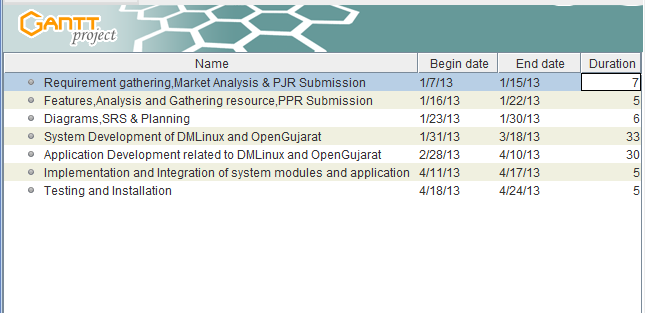
\includegraphics[scale=0.6] {gantt1.png}
  \caption[Project Planning]{Project Plan}
\end{center}
\end{figure}
\begin{figure}[h]
\begin{center}
  % Requires \usepackage{graphicx}
  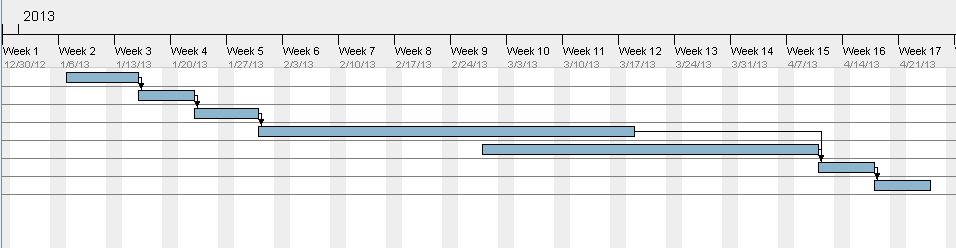
\includegraphics[scale=0.4] {gantt2.png}\\
  \caption[Timeline]{Project Plan - Timeline}
\end{center}
\end{figure}


\chapter{System Analysis}
\section{Feasibility Study}
The Objective of the Feasibility study:
The purpose of the Feasibility study is to find out if an information system project can be done and to suggest possible alternate solution. Feasibility study of the system is very important stage during the system design. Feasibility study is a test of a system proposal according to its workability impact on the organization, ability to meet user needs, and effective use of resources. (Hardware, Software, or other equipments), It is also use to determine whether the system gives benefit to people or society or not? Feasibility study decides whether the proposed system is properly developed or not or it properly work as per the expectation of the company or not.

Need for Feasibility Study:
A feasibility study is written approach to evaluating your idea and can help you identify:
\begin{itemize}
\item If your idea is viable or not
\item Useful facts and figures to aid decision-making
\item Alternative approaches and solutions to putting your idea into practice
\end{itemize}
There are many reasons why new community ventures fail, but lack of planning and research is the main one. As you plan, your knowledge of your market, customers and the environment in which you will work will grow. This process considers all areas of your idea and ensures you have something concrete on paper.

What does a feasibility study involve?

It can involve some or all of the following:
\begin{itemize}
\item An assessment of the current market
\item An assessment of your potential position in the market
\item An evaluation of the possible options for entry into the market
\item A short list of the possible options
\end{itemize}
There are some aspects in feasibility study portion of the preliminary investigation.
\begin{enumerate}
  \item Technical Feasibility.
  \item Economic Feasibility.
  \item Operational Feasibility.
  \item Social Feasibility.
  \item Legal Feasibility
  \item Time Feasibility of the project.
\end{enumerate}

\subsection{Technical feasibility}
A large part of determining resources has to do with assessing technical feasibility. It must be find out whether current technical resources can be upgraded or added in a manner that fulfills the request  under consideration. It is willing to improve its technical abilities of the project will be handled on the computerized concept so it has to improve some hardware and software abilities to maintain this system and it billing to improve and give all the supported facilities.
Here, the Proposed System which is to be developed requires Hardware as well as Software Resources.
A Hardware requirement includes PC with 40GB Hard disk and 1GB RAM.  Software requirement includes Java.
File requirement: Shape Files or geo referenced .jpg or .tiff file
It may be affordable for any organization to employee new professional thus, the requirement makes it technical feasible.

\subsection{Economic feasibility}
Economic feasibility looks at the financial aspects of the project. Economic feasibility concerns with the returns from the investments in a project. It determines whether it is worthwhile to invest the money in the proposed system. It is not worthwhile spending a lot of money on a project for no returns.
To carry out an economic feasibility for a system, it is necessary to place actual money value against any purchases or activities needed to implement the project.
The proposed system that is going to develop its benefit is indirect benefit and cost is direct cost that is to be paid. It costs for its development and hiring of the Server space. But it gives indirect benefit to businessman’s tourist etc.

\subsection{Operational feasibility}
The System will hold good GUI facilities which attract the user to use the System. The System will be developed using new technologies so the user will even get a chance work with and learn new technology and environment.
Company is having sufficient employees for designing, implementing, testing, deploying and the training the employee to uses that system.
In the system operational feasibility checks, whether the user who is going to use the system is able to work with the software’s with which the system is coded and also the mind of the user going to use the system. If the user does not understand or is able to work on the system further development is of waste.

\subsection{Social feasibility}
The System is going to be developed is it beneficial to society? Yes, as this System gives the details of the district to the user and admin and user can edit the shape files and get better view of the map also by having charts cam save as image which can be useful as map
\subsection{Legal feasibility}
The Proposed System should be such that the System do not misguide or gives wrong information to user. The System should give proper information and should be reliable source of information to user.
\subsection{Time feasibility}
The Proposed System is a Desktop  Application so it will take some duration of time to satisfy the objective of completing the System (Application). The duration that is allocated to develop the System is quite feasible in respect to time. 4 months is enough to develop System.

\section{Requirement Analysis}
\subsection{Facts finding techniques}
The client in most cases is not sure of what exactly is desired and has a poor understanding of the computing environment
\begin{itemize}
\item Inception of the Project
\item Basic Elicitation
\begin{itemize}
\item Problems of Scope
\item Problems of Understanding
\item Problems of Volatility
\end{itemize}
\item Elaboration
\item Negotiation
\item Specification
\item Validation
\item Management (Continuous)
\item The  following  techniques  are  present  unambiguously  throughout  the  project  and possess enormous power with regard to requirement gathering.
\end{itemize}

\subsubsection{Interview}
The requirement analysis phase begins after the inception of the project.
The first phase of interviews is mainly a kind of informal discussions with the client. In this phase the analysts who are the evangelists in the process of requirement elicitation generally do the following:
\begin{itemize}
\item Ask a set of Informal  Context Free Questions regarding  the system.
\item Talk   through   with   the   client   to   know   his   intention   with   regard   to   the project.
\item Define  a  business  case  for  the  idea  along  with  the  performance  of  certain kind of market analysis.
\item Identify a working description of the project’s scope.
\end{itemize}
The later phases of interviews involve the following kind of facets:
\begin{itemize}
\item Discussion  on  the  Division  of  the  entire  thing  into  manageable  and  doable modules.
\item Module wise interviews with the various personnel  involved.
\item Certain   kind   of   debatable   presentations   which   may   be   clubbed   with brainstorming or prototyping  sessions.
\end{itemize}
This mode of requirement gathering is the one that provides the maximum amount of information regarding the  project and hence is used very effectively. This mode can turn into all various forms ranging from strict one room interviews to large debatable discussions.

\subsubsection{Questionnaire}
This mode of requirement elicitation is generally employed during change management and while laying out basic system explanations.
Questionnaires used in the project are framed keeping into mind the following things:
\begin{itemize}
\item Amount and the kind  of information to be extracted  through this     channel.
\item The kind of stake holder to whom the questionnaire is addressed.
\item The reusability and  abstractness of these questionnaires.
\end{itemize}
\subsubsection{Record Review}

The records analyzed by me  were mainly the following:
\begin{itemize}
\item Software Design Document
This gave me the actual requirements of the GUI plus the backend logic right till statement of logical queries which may be employed in some or the other form. It also incorporated the sample GUI so that any  changes to the prototypes submitted earlier can be  checked and tracked.
\item Technical SRS (with Business Analysis)
This was a typical  SRS  that gave me the specific requirements along with the Business rules that need to be employed.
\item Class Diagrams
The class diagram made me understand the entire architecture that was employed and allowed me to extend it in my system.
\end{itemize}
\subsubsection{Observation}
This is also the method employed very widely in the project being developed. The  developers working   onsite generally engage in the observation of the following things:
\begin{itemize}
\item Work Environment of the organization.
\item The technical expertise of the employees of the organization.
\item The volume of customers entertained.
\item The kind of system expected.
\item The  resistance  in  the  organization  due   while   the   organization  gets   the system installed.
\item The usage of any of the available systems.
\end{itemize}
During the continuous management phase that starts once the system is installed and is running the   observation regarding system usage, system inconveniences and system benefits is carried  out.

\subsection{Data Flow Diagrams}
\begin{figure}[h]
\begin{center}
  % Requires \usepackage{graphicx}
  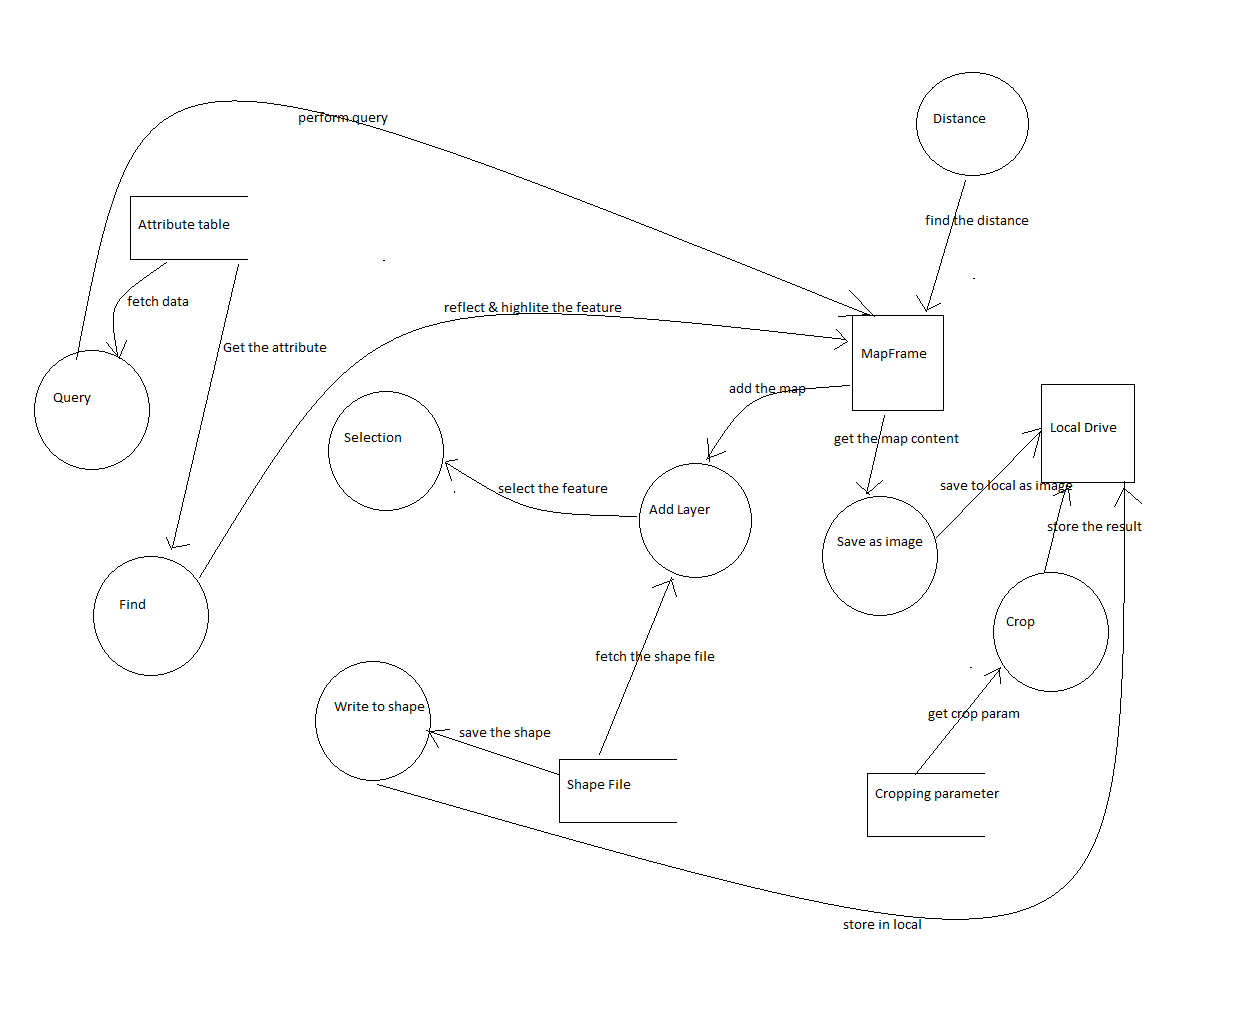
\includegraphics [scale=0.43] {DataFlow.png}
  \caption[Data Flow Diagram]{Data flow diagram of desktop GIS application}
\end{center}
\end{figure}
